\documentclass[border=10pt]{standalone}
\usepackage{pgfplots}
\pgfplotsset{compat=1.18}
\begin{document}
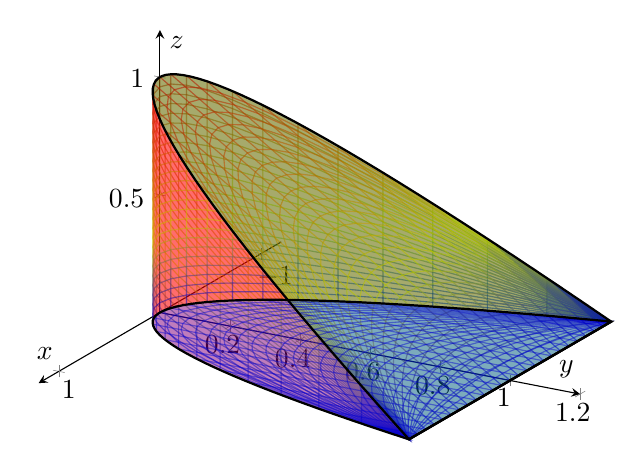
\begin{tikzpicture}
\begin{axis}[
    view={120}{30},
    axis lines=middle,
    xlabel={$x$}, ylabel={$y$}, zlabel={$z$},
    xmin=-1.2, xmax=1.2,
    ymin=0, ymax=1.2,
    zmin=0, zmax=1.2,
    width=10cm, height=8cm,
    grid=major,
]
% parabolic cylinder y=x^2, 0<=z<=1-x^2
\addplot3[
    surf, opacity=0.35,
    domain=-1:1, domain y=0:1,
    samples=25, samples y=25,
    color=red,
] ({x}, {x^2}, {y*(1-x^2)});

% top plane z=1-y over x^2<=y<=1
\addplot3[
    surf, opacity=0.35,
    domain=-1:1, domain y=0:1,
    samples=25, samples y=25,
    color=green!70!black,
] ({x}, {x^2 + y*(1-x^2)}, {(1-y)*(1-x^2)});

% bottom plane z=0
\addplot3[
    surf, opacity=0.25,
    domain=-1:1, domain y=0:1,
    samples=25, samples y=25,
    color=blue,
] ({x}, {x^2 + y*(1-x^2)}, {0});

% boundary curves
\addplot3[domain=-1:1, samples=60, thick, black] ({x},{x^2},{0});
\addplot3[domain=-1:1, samples=60, thick, black] ({x},{x^2},{1-x^2});
\addplot3[domain=-1:1, samples=2, thick, black] ({x},{1},{0});
\end{axis}
\end{tikzpicture}
\end{document}